\documentclass{article}
\usepackage[review]{log_2026}   % anonymous submission to proceedings track

\usepackage{booktabs}
\usepackage{multirow}
\usepackage{amsfonts}
\usepackage{amsmath}
\usepackage{graphicx}
\usepackage{subcaption}
\usepackage{algorithm}
\usepackage{algpseudocode}
\usepackage{threeparttable}
\usepackage{array,color}
\usepackage{url}
\usepackage[numbers,compress,sort]{natbib}

\title[Graph-Weighted CCA for Inductive Attributed Graph Embedding]
      {Graph-Weighted Canonical Correlation Analysis: A Closed-Form Method for Inductive Attributed Graph Embedding}

\author[Anonymous]{%
Anonymous Authors\\
Anonymous Institution\\
\email{anonymous@example.com}}

\begin{document}
\maketitle

\begin{abstract}
We introduce \textbf{Graph-Weighted Canonical Correlation Analysis (GW-CCA)},
a closed-form method for inductive attributed graph embedding. GW-CCA
modifies classical CCA by inserting a random-walk graph similarity matrix
into the cross-covariance, so that cross-view alignment is weighted by
graph proximity rather than restricted to the same node across views. For
attributed graphs with a single feature matrix, we construct the second
view by multi-hop graph propagation of the features, yielding a linear,
non-iterative method that requires only a feature-dimensional
eigendecomposition rather than GNN training. Across five inductive
benchmarks, GW-CCA is competitive with or stronger than representative
GNN and graph self-supervised baselines for node classification, and
achieves the best link-prediction performance in our evaluation while
requiring orders of magnitude less training time. The method recovers
standard CCA when graph weighting is removed and provides a simple
alternative to deep graph self-supervised learning for large-scale
inductive representation learning.
\end{abstract}

\section{Introduction}
\label{sec:intro}

Graph representation learning maps nodes to low-dimensional vectors that
encode both graph structure and node attributes, enabling downstream tasks
such as node classification and link prediction. In the \emph{inductive}
setting, a model trained on one graph, or on a training subgraph, must
generate representations for previously unseen nodes. Classical shallow
methods such as DeepWalk~\citep{perozzi2014deepwalk},
node2vec~\citep{grover2016node2vec}, LINE~\citep{tang2015line}, and their
matrix-factorisation interpretations~\citep{qiu2018network} are efficient,
but they learn per-node embeddings and are therefore transductive unless
retrained or equipped with an additional out-of-sample extension.

Recent progress in inductive graph representation learning has instead
been driven largely by deep self-supervised graph neural networks,
including contrastive~\citep{zhu2020deep,thakoor2022bgrl},
mutual-information~\citep{velickovic2019deep,peng2020graph},
CCA-inspired~\citep{zhang2021ccassg,bielak2022graphbt}, and
masked-autoencoding methods~\citep{hou2023graphmae2}. Although effective,
these methods require stochastic optimisation, augmentation design,
learning-rate schedules, epoch tuning, and substantial GPU training time.
Linear propagation methods such as SGC~\citep{wu2019simplifying}, and its
extensions SIGN~\citep{frasca2020sign} and
S\textsuperscript{2}GC~\citep{zhu2021ssgc}, avoid deep message passing and
are inductive by construction --- but they are typically used as
supervised task-specific encoders, not as closed-form unsupervised
multiview embedding methods. This raises a natural question: can inductive
attributed graph embeddings be learned with a simpler closed-form method
while still exploiting graph structure?

We answer this question with \textbf{Graph-Weighted Canonical Correlation
Analysis (GW-CCA)}\footnote{Code and reproducibility artifacts:
\url{https://anonymous.4open.science/r/gw-cca-6151}.}, a closed-form
method for inductive attributed graph embedding. Standard CCA learns linear projections that align paired points
$x_1^{(i)}$ and $x_2^{(i)}$ from two views by maximising
$\mathrm{Tr}(W^\top X_1^\top X_2 H)$. GW-CCA replaces the ordinary
cross-covariance $X_1^\top X_2$ with a graph-weighted cross-covariance
$X_1^\top M X_2$, where $M_{ij}$ measures random-walk similarity between
nodes $v_i$ and $v_j$ (e.g., $M = (P + P^2)/2$ with $P = D^{-1}A$)
(Figure~\ref{fig_1}). Node $i$'s representation in one view is thus
aligned with node $j$'s representation in the other view in proportion to
their graph proximity, rather than only same-index pairs. For attributed
graphs with a single feature matrix $X$, we construct the second view
deterministically as $X_2 = \widehat{P}^K X$, where
$\widehat{P} = (D + I_n)^{-1}(A + I_n)$ is the self-looped,
row-normalised adjacency (an SGC-inspired propagation kernel, a
row-stochastic self-loop variant of the symmetric kernel of
\citet{wu2019simplifying}). GW-CCA then solves a single
feature-dimensional ($p \times p$) decomposition to obtain the
projections; the method is non-iterative, deterministic, and inductive by
construction, embedding unseen nodes by propagating their features on the
observed graph and applying the learned projections. In particular, GW-CCA
is a strict generalisation of standard
CCA~\citep{hotelling1992relations}, recovered when $M = I_n$.

Across five inductive benchmarks --- ogbn-arxiv, Reddit, Yelp,
ogbn-products, and PPI --- GW-CCA is competitive with or stronger than
representative GNN and graph self-supervised baselines for node
classification, and achieves the best link-prediction performance in our
evaluation, while requiring orders of magnitude less encoder-training
time on a single CPU (Table~\ref{tab:efficiency}). These results suggest
that graph-weighted closed-form CCA can provide a simple and effective
alternative to deep graph self-supervised learning for large-scale
inductive attributed graph embedding.

\paragraph{Contributions.}
\begin{itemize}
\item A \emph{graph-weighted cross-covariance} objective
(\S\ref{sec:approach}) that turns CCA into an inductive attributed graph
embedding method, with standard CCA recovered when $M = I_n$.
\item A closed-form solver based on a single feature-dimensional
($p \times p$) decomposition, together with a deterministic two-view
construction $X_2 = \widehat{P}^K X$ for standard attributed graphs
(\S\ref{sec:apply}).
\item An empirical study on five inductive benchmarks under a strict
inductive protocol, showing strong node-classification performance and
leading link-prediction performance against representative deep graph SSL
baselines (\S\ref{sec:exp}).
\item A precise positioning against CCA-inspired graph
SSL~\citep{zhang2021ccassg,bielak2022graphbt}: GW-CCA inserts graph
structure directly into the cross-covariance rather than using it as an
augmentation-invariance loss (\S\ref{sec:approach:ssl});
Appendix~\ref{app:reg-cca} additionally contrasts GW-CCA with
graph-regularised CCA~\citep{yuan2014graph,chen2018canonical,chen2018canonical2},
which uses Laplacian penalties.
\end{itemize}

\begin{figure}[t]
  \centering
  \begin{subfigure}[b]{0.36\linewidth}
    \centering
    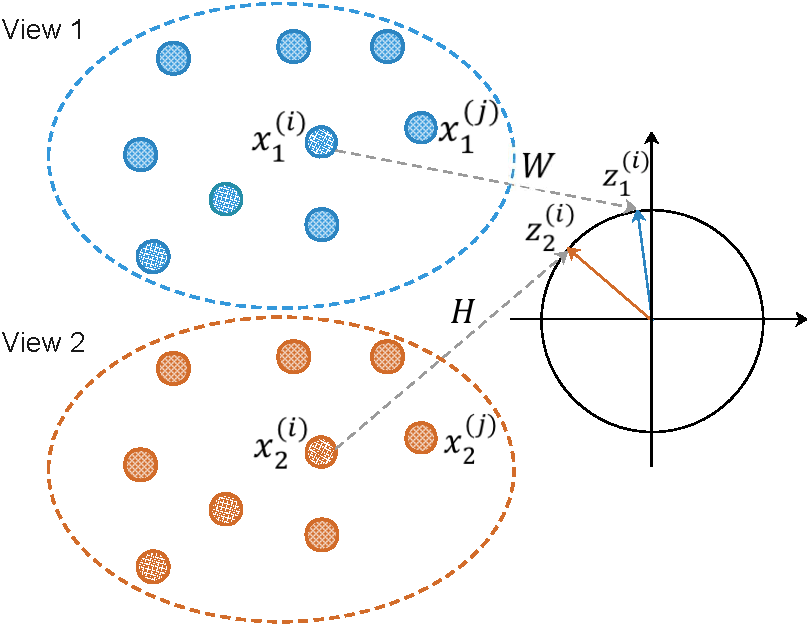
\includegraphics[width=\linewidth]{figures/CCA.pdf}
    \caption{Standard CCA}
    \label{fig_1_a}
  \end{subfigure}\hskip 0.1in
  \begin{subfigure}[b]{0.42\linewidth}
    \centering
    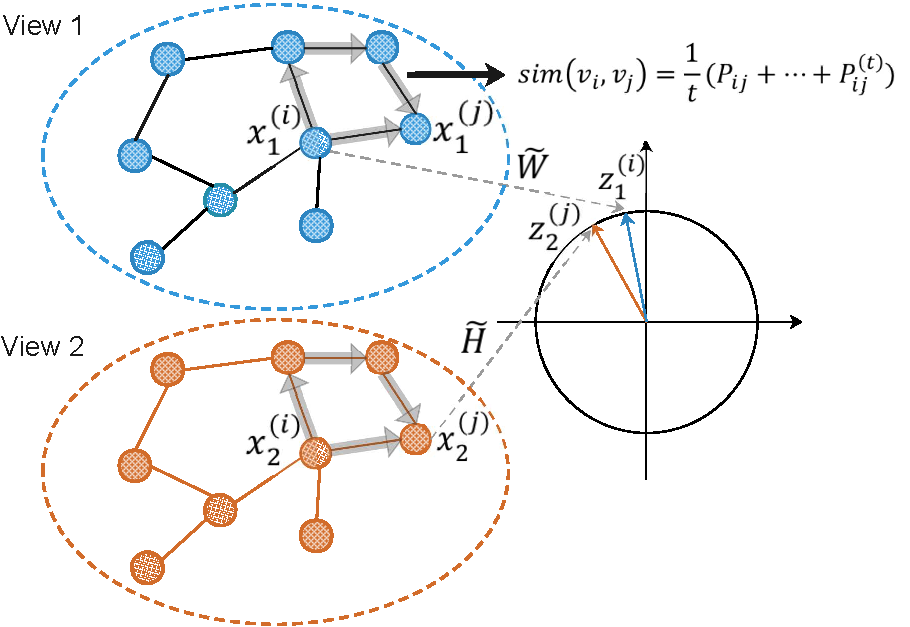
\includegraphics[width=\linewidth]{figures/DWA_CCA.pdf}
    \caption{GW-CCA}
    \label{fig_1_b}
  \end{subfigure}
  \caption{Standard CCA vs.\ GW-CCA.
  (a) Standard CCA aligns same-index pairs across two views after linear
  projection.
  (b) GW-CCA aligns cross-view node pairs according to graph similarity:
  larger $M_{ij} = \mathrm{sim}(v_i, v_j)$ gives greater weight to the
  dot-product alignment ${z_1^{(i)}}^\top z_2^{(j)}$.}
  \label{fig_1}
\end{figure}

\section{Background}
\label{sec:background}

\subsection{Inductive Attributed Graph Embedding}
Let $G = (V, E)$ be a graph with $n = |V|$ nodes, adjacency matrix
$A \in \mathbb{R}^{n \times n}$, and node feature matrix
$X \in \mathbb{R}^{n \times p}$. Attributed graph embedding learns a
representation $z^{(i)} \in \mathbb{R}^d$ for each node that captures
both its attributes $x^{(i)}$ and its graph context. In the
\emph{inductive} setting, the embedding rule must generalise to unseen
nodes without learning a separate lookup vector for each training node:
a method trains on a graph or training subgraph and later embeds new
nodes using their features and observable incident edges, without
retraining. This excludes purely transductive methods such as DeepWalk
and node2vec~\citep{perozzi2014deepwalk,grover2016node2vec} unless an
explicit out-of-sample extension is added.

\subsection{Canonical Correlation Analysis}
Given two paired feature matrices $X_1, X_2 \in \mathbb{R}^{n \times p}$
(the setting used by GW-CCA in \S\ref{sec:apply}, where both views share
the same $p$-dimensional feature space), CCA learns linear projections
$W, H \in \mathbb{R}^{p \times d}$ that maximise the cross-view
cross-covariance
\begin{equation}\label{eq:cca-2}
\arg\max_{W, H}\ \mathrm{Tr}(W^\top X_1^\top X_2 H),
\quad \text{s.t.}\quad W^\top X_1^\top X_1 W = I_d,\ H^\top X_2^\top X_2 H = I_d;
\end{equation}
see~\citet{hardoon2004canonical} for the derivation from the correlation
coefficient. With $Z_1 = X_1 W$ and $Z_2 = X_2 H$, CCA projects paired
points into representations whose cosine similarity
${z_1^{(i)}}^\top z_2^{(i)}$ is maximised (Figure~\ref{fig_1_a}).
Eq.~\ref{eq:cca-2} admits a closed-form solution via a singular value
decomposition of a $p \times p$ matrix built from the covariances of
$X_1$ and $X_2$; CCA is thus inductive and efficient when $p \ll n$. It
captures only linear relationships and treats each same-index pair
$(x_1^{(i)}, x_2^{(i)})$ symmetrically --- discarding any additional
pairing information such as graph similarity, which \S\ref{sec:approach}
addresses by inserting a graph similarity matrix $M$ into the
cross-covariance of Eq.~\ref{eq:cca-2}.

\section{Graph-Weighted CCA}
\label{sec:approach}

\subsection{Objective}
\label{sec:approach:objective}

Standard CCA aligns paired points $(x_1^{(i)}, x_2^{(i)})$ under the
assumption that same-index correspondence is the only pairing information.
On attributed graphs we have richer pairing information --- graph similarity
$M_{ij}$ between nodes $v_i$ and $v_j$ --- that CCA discards. GW-CCA
generalises CCA by using $M$ to re-weight the cross-view alignment, so that
structurally similar nodes are pulled together across views.

Concretely, given two views of data $X_1$ and $X_2$, GW-CCA learns a pair of
projections $\widetilde{W}, \widetilde{H}$ by solving
\begin{equation}\label{eq:gcca}
\arg\max_{\widetilde{W}, \widetilde{H}}\ \mathrm{Tr}(\widetilde{W}^\top X_1^\top M X_2 \widetilde{H}),\
\text{s.t.}\ \widetilde{W}^\top X_1^\top X_1 \widetilde{W} = I_d,\ \widetilde{H}^\top X_2^\top X_2 \widetilde{H} = I_d,
\end{equation}
where $M \in \mathbb{R}^{n\times n}$ defines pairwise node similarity in the
original graph, i.e., $M_{ij} = \mathrm{sim}(v_i, v_j)$. Two special cases
are worth noting: setting $M = I_n$ recovers standard
CCA~\citep{hotelling1992relations} (Eq.~\ref{eq:cca-2}); and, as we make
precise in \S\ref{sec:apply}, our two-view construction
$X_2 = \widehat{P}^K X$ reuses an SGC-style~\citep{wu2019simplifying}
propagation kernel, so an SGC-style spectral filter appears inside GW-CCA.

Writing the projected representations as
$z_1^{(i)} = \widetilde{W}^\top x_1^{(i)}$ and
$z_2^{(j)} = \widetilde{H}^\top x_2^{(j)}$ (Figure~\ref{fig_1_b}),
The objective of Eq.~\ref{eq:gcca} admits an equivalent pointwise
expansion over cross-view node pairs (Appendix~\ref{app:derivations:pointwise}):
\begin{equation}\label{eq:gcca-rep}
\mathrm{Tr}\!\left(\widetilde{W}^\top X_1^\top M X_2 \widetilde{H}\right)
\;=\; \sum_{i,j=1}^{n} M_{ij}\, {z_1^{(i)}}^\top z_2^{(j)},
\end{equation}
This makes the role of $M$ explicit as a change to CCA's pairing structure:
standard CCA is the $M = I_n$ case, which assigns weight $1$ only to
same-index pairs $(i, i)$ and weight $0$ to all cross-node pairs. GW-CCA
replaces that identity pairing with a graph-dependent soft pairing --- node
$i$ in view~1 aligns with node $j$ in view~2 whenever $M_{ij}$ is large ---
so structurally similar nodes are pulled together across views. The
whitening constraints of Eq.~\ref{eq:gcca} remain in force;
Eq.~\ref{eq:gcca-rep} rewrites only the objective. After solving
Eq.~\ref{eq:gcca}, we concatenate $X_1 \widetilde{W}$ and
$X_2 \widetilde{H}$ to form the final $n \times 2d$ node representation
matrix. The projections are linear in the features, but $M$ is a
polynomial of the adjacency matrix (\S\ref{sec:apply}), so multi-hop graph
structure enters the eigenvalue problem through $M$ --- unlike standard CCA
applied to the same two views, which would ignore $M$ entirely. How the
two views $X_1, X_2$ and the similarity $M$ are constructed from a
standard attributed graph with one feature matrix appears in
\S\ref{sec:apply}.

\subsection{Closed-Form Solution}
\label{sec:approach:solution}

Eq.~\ref{eq:gcca} assumes $X_k^\top X_k$ is non-singular; when it is not
(e.g., Yelp in \S\ref{sec:exp}), we solve the ridge-regularized variant
obtained by replacing $X_k^\top X_k$ with
$C_{kk} = X_k^\top X_k + \lambda_k I_p$ ($\lambda_k \geq 0$) in both the
whitening constraints and the closed form below --- setting $\lambda_k = 0$
recovers Eq.~\ref{eq:gcca}, and \S\ref{sec:exp} shows GW-CCA is insensitive
to $\lambda_1 = \lambda_2 = \lambda$. Let $T = X_1^\top M X_2$. A whitening
change of variables reduces this (regularized) Eq.~\ref{eq:gcca} to a
truncated singular value decomposition (Appendix~\ref{app:derivations:svd}):
\begin{equation}\label{eq:gcca-svd}
C_{11}^{-1/2}\, T\, C_{22}^{-1/2} = U\, \Sigma\, V^\top,
\qquad
\widetilde{W} = C_{11}^{-1/2} U_{:,1:d},
\qquad
\widetilde{H} = C_{22}^{-1/2} V_{:,1:d},
\end{equation}
where $U_{:,1:d}$ and $V_{:,1:d}$ hold the top-$d$ left and right singular
vectors and $\Sigma_{ii}$ is the $i$-th singular value of the whitened
graph-weighted cross-moment matrix --- an $M$-weighted alignment score
bounded by $\|M\|_2$. When $M = I_n$ (and features are centered) this
reduces to the classical canonical correlation, bounded in $[0, 1]$; for
general $M$ (in particular, non-symmetric row-stochastic $P$ on hub-heavy
graphs) $\|M\|_2$ can exceed $1$, so we refer to the $\Sigma_{ii}$ as
$M$-weighted alignment scores rather than correlations. In practice
$C_{kk}^{-1/2}$ is applied implicitly via a Cholesky factorisation of
$C_{kk}$ --- never formed as an explicit inverse --- and only the top-$d$
singular triplets are computed. Three dense $p \times p$ matrices
($C_{11}$, $C_{22}$, and the cross term $T = X^\top(MX_2)$) plus the two
Cholesky factors $L_1, L_2$ are materialised; the whitened SVD target
$C_{11}^{-1/2} T C_{22}^{-1/2}$ itself is never formed explicitly, being
accessed only through triangular solves against $L_1, L_2$.
Concretely, the SVD is taken of $L_1^{-1} T\, L_2^{-\top}$ and the
projections reconstructed via $\widetilde{W} = L_1^{-\top} U_{:,1:d}$,
$\widetilde{H} = L_2^{-\top} V_{:,1:d}$, which yields a whitened solution
differing from Eq.~\ref{eq:gcca-svd} by a rotation and identical
singular values. An equivalent generalised eigenvalue
formulation on $(T\, C_{22}^{-1}\, T^\top,\ C_{11})$ recovers the same
$\widetilde{W}$ up to sign; we adopt the SVD form because it yields both
projections from a single decomposition and is better conditioned than
the generalised eigenvalue formulation.

\subsection{Comparison to CCA-Inspired Graph Self-Supervised Learning}
\label{sec:approach:ssl}
A more recent line of work uses CCA-style objectives as \emph{losses} for
training graph neural networks in a self-supervised
manner~\citep{zhang2021ccassg,bielak2022graphbt}. CCA-SSG
\citep{zhang2021ccassg} generates two augmented views of an input graph and
trains a GNN encoder to (i)~align the two views' representations and
(ii)~decorrelate feature dimensions, mirroring the invariance and whitening
constraints of CCA. Graph Barlow Twins~\citep{bielak2022graphbt} adopts the
closely related Barlow-Twins cross-correlation objective for the same
purpose. GW-CCA differs from these methods in three ways.
\emph{(i)~Shallow, closed-form solver vs.\ SGD.} We solve the CCA
problem in closed form via SVD; there is no encoder to train,
no augmentation schedule, and no learning-rate/epoch tuning. Consequently,
GW-CCA is two to three orders of magnitude faster than SSL baselines in our
experiments (Table~\ref{tab:efficiency}), and its output is deterministic.
\emph{(ii)~CCA as solver vs.\ CCA as loss.} CCA-SSG and G-BT use a
CCA-inspired \emph{loss} to train a neural encoder; GW-CCA \emph{is} CCA,
with the graph inserted into the cross-covariance and solved by
eigen-decomposition. \emph{(iii)~Structural weighting vs.\ same-index
invariance.} CCA-SSG/G-BT align the same node's representations across two
augmented views (encouraging augmentation invariance). GW-CCA aligns
\emph{cross-node} pairs $(i,j)$ weighted by graph similarity $M_{ij}$
(Eq.~\ref{eq:gcca-rep}), so it explicitly encourages structurally similar
nodes---not just the same node under two random augmentations---to have
similar cross-view representations.

Orthogonal to these graph-focused extensions, a separate line of work
non-linearises CCA itself: Kernel CCA~\citep{hardoon2004canonical} maps
inputs to a reproducing-kernel Hilbert space, Deep
CCA~\citep{andrew2013deep} learns two deep neural encoders in place of the
linear projections, and DCCAE~\citep{wang2015deep} adds an autoencoder
regulariser. GW-CCA differs on the opposite axis: it keeps the projections
strictly linear but reweights the cross-covariance by graph similarity, so
multi-hop graph structure enters through $M$ rather than through a deeper
encoder --- and the whole system remains closed-form, with no encoder
training or augmentation schedule.

\section{Instantiation for Attributed Graphs}
\label{sec:apply}

Section~\ref{sec:approach} defines GW-CCA for arbitrary $(X_1, X_2, M)$;
we now construct each from an attributed graph with feature matrix $X$
and adjacency $A$.

\subsection{Graph-Aware View Construction}
Attributed graphs come with a single feature matrix $X$; we set $X_1 = X$
and construct a second view $X_2 = f(X)$ deterministically from $X$ and the
graph, using a graph-aware map
$f : \mathbb{R}^{n \times p} \rightarrow \mathbb{R}^{n \times p}$. To
incorporate graph information, we use the graph convolution
of~\citet{wu2019simplifying}:
\begin{equation}\label{eq:f}
X_2 = f(X) = \widehat{P}^K X,
\end{equation}
where $\widehat{P} = (D + I_n)^{-1}(A + I_n)$ is a normalised adjacency matrix and
$K$ is the number of propagation steps. As noted in
\S\ref{sec:approach:objective}, this is a row-stochastic variant of
SGC's~\citep{wu2019simplifying} propagation kernel: the $i$-th row of
$X_2$ is a $K$-hop weighted aggregate
of neighbouring features, so the second view carries local graph topology
into the feature space, and CCA on $(X, \widehat{P}^K X)$ becomes a
graph-aware alignment problem. Computing $X_2$ takes $\mathcal{O}(K|E|p)$
time when $\widehat{P}$ is sparse. The propagation kernel $\widehat{P}$
and the similarity kernel used in \S\ref{sec:apply:M} play distinct
roles in the objective. $\widehat{P}$ smooths features into a second
view $X_2 = \widehat{P}^K X$ that CCA aligns with $X_1 = X$ (row
normalisation with self-loops, for SGC-style low-pass filtering), while
$P = D^{-1}A$ (without self-loops) defines a pair-weight matrix $M$
that reweights which cross-view row pairs contribute to
Eq.~\ref{eq:gcca}. Both kernels are low-order polynomials of
row-normalised adjacencies and act as low-pass filters emphasising
neighbourhood-smooth feature components; GW-CCA then selects
projections whose graph-filtered cross-view alignment is largest ---
the same low-pass regime that motivates
SGC~\citep{wu2019simplifying}, now driving the CCA objective rather
than a supervised loss.

\subsection{Random-Walk Pair Weights}
\label{sec:apply:M}
We use the truncated random-walk similarity
\begin{equation}\label{eq:M}
M = \frac{P + P^2}{2}, \qquad P = D^{-1}A,
\end{equation}
which encodes two deliberate design decisions.

\paragraph{Row-normalised, not symmetric-normalised.}
We take $P = D^{-1}A$ rather than the self-looped $\widehat{P}$ used for
the second view because $[P^r]_{ij}$ is a proper transition probability --- the
probability that an $r$-step random walk from $v_i$ ends at $v_j$. Symmetric
normalisation mixes this with degree factors and loses the random-walk
interpretation that motivates using $M$ as a similarity in the first place.
The two kernels' complementary roles play together in
\S\ref{sec:apply:special}. A symmetric normalisation could also be used
when a bounded spectral norm is desired, but it loses the direct
random-walk interpretation. We use the row-stochastic form throughout
because $M$ is intended to encode transition-based proximity.

\paragraph{Truncation at $r = 2$.}
We choose $T = 2$ because the GW-CCA objective uses $M$ only to weight
cross-view pairs: first-order (direct-neighbour) proximity aligns
connected nodes, and second-order (shared-neighbour) proximity aligns
nodes with overlapping neighbourhoods --- both are informative for
downstream tasks. Higher powers $P^r$ spread mass over increasingly
distant nodes and can blur class-relevant local structure, at additional
propagation cost. This is consistent with LINE~\citep{tang2015line},
which explicitly models the same two orders, and with DeepWalk's implicit
target: \citet{qiu2018network} show DeepWalk factorises
$\log\!\big(\mathrm{vol}(G) \cdot \tfrac{1}{T}\sum_{r=1}^{T} P^r \cdot D^{-1}\big)$,
so $T = 2$ (dropping the log/degree scaling) recovers $M$ up to a
constant. \S\ref{sec:exp} confirms that raising $T$ beyond $2$ does not
improve downstream performance. Although $P^2$ can be much denser than
$P$ in graphs with high-degree hubs, GW-CCA never materialises $M$
explicitly; it applies $M$ to $X_2$ via two sparse SpMV rounds,
$M X_2 = \tfrac{1}{2}(P X_2 + P(P X_2))$, at $\mathcal{O}(|E| p)$ cost
regardless of $P^2$'s density --- the property the complexity analysis in
\S\ref{sec:complexity} actually relies on.

\subsection{Special Cases and Ablations}
\label{sec:apply:special}

Table~\ref{tab:special-cases} places GW-CCA inside the design space
$(X_1, X_2, M)$. Setting $M = I_n$ recovers standard CCA on the chosen two
views; combining $M = I_n$ with the propagated view $X_2 = \widehat{P}^K X$
yields the CCA$^\ast$ baseline reported in
Tables~\ref{tab:node-cls}--\ref{tab:link-pred}, which is the cleanest
ablation of GW-CCA: everything except the graph-weighted cross-covariance
is held fixed, so any margin of GW-CCA over CCA$^\ast$ is attributable to
$M$ alone.

\begin{table}[ht]
\caption{Special cases of Eq.~\ref{eq:gcca} on the two-view construction
$(X, \widehat{P}^K X)$. CCA$^\ast$ is the graph-unweighted counterpart of
GW-CCA; GW-CCA replaces the ordinary cross-covariance with a
graph-weighted one.}
\label{tab:special-cases}
\centering
\begin{tabular}{cccl}
\toprule
$X_1$ & $X_2$ & $M$ & Method \\
\midrule
$X$               & $\widehat{P}^K X$ & $I_n$            & CCA$^\ast$ (Table~\ref{tab:node-cls} baseline) \\
$X$               & $\widehat{P}^K X$ & $(P + P^2)/2$    & \textbf{GW-CCA} \\
\bottomrule
\end{tabular}
\end{table}

\subsection{Algorithm and Inductive Inference}
\label{sec:apply:algorithm}

Algorithm~\ref{alg_1} lays out both phases in a single block. Training uses
only the training-subgraph adjacency $A$ (edges among training nodes) to
learn the projection pair $(\widetilde{W}, \widetilde{H})$; inductive
inference then applies them to the full observed graph $(A', X')$ ---
containing $(A, X)$ as its training-node-induced subgraph plus previously
unseen test nodes and any edges incident to them --- without retraining or
fine-tuning. This matches the standard inductive protocol
of~\citet{hamilton2017inductive}: the graph structure among test nodes is
observable at inference time, but their labels are not, and no test-node
features or edges enter training.

\begin{algorithm}[t]
\caption{GW-CCA: training and inductive inference}
\label{alg_1}
\begin{algorithmic}[1]
\Statex \textbf{Training phase.} Inputs: training-subgraph adjacency $A$, training features $X \in \mathbb{R}^{n \times p}$, embedding dim $d$, propagation depth $K$, ridge $\lambda \geq 0$. Returns $\widetilde{W}, \widetilde{H} \in \mathbb{R}^{p \times d}$.
\State $P \gets D^{-1} A$;\quad $\widehat{P} \gets (D + I_n)^{-1}(A + I_n)$
\State $X_2 \gets \widehat{P}^K X$ \Comment{$K$ sparse SpMVs; do not materialise $\widehat{P}^K$}
\State $M X_2 \gets \tfrac{1}{2}\bigl(P X_2 + P(P X_2)\bigr)$ \Comment{apply $M = (P + P^2)/2$ to $X_2$ via two sparse SpMV rounds ($\mathcal{O}(|E|p)$); do not materialise $M$ or $P^2$}
\State $C_{11} \gets X^\top X + \lambda I_p$;\ \ $C_{22} \gets X_2^\top X_2 + \lambda I_p$;\ \ $T \gets X^\top (M X_2)$
\State Cholesky factorise $C_{kk} = L_k L_k^\top$ for $k \in \{1, 2\}$, giving $C_{kk}^{-1/2}$ implicitly
\State $U, \Sigma, V \gets \textsc{TruncatedSVD}\!\left(C_{11}^{-1/2}\, T\, C_{22}^{-1/2},\ \text{rank}=d\right)$
\State $\widetilde{W} \gets C_{11}^{-1/2}\, U$;\ \ $\widetilde{H} \gets C_{22}^{-1/2}\, V$ \Comment{Eq.~\ref{eq:gcca-svd}}
\Statex \textbf{Inductive inference.} Given the full observed graph $A'$ and features $X'$ --- including previously unseen test nodes and their incident edges, but \emph{no test labels} --- return $Z' \in \mathbb{R}^{n' \times 2d}$ for every node of $A'$:
\State $\widehat{P}' \gets (D' + I_{n'})^{-1}(A' + I_{n'})$
\State $X_2' \gets \widehat{P}'^K X'$ \Comment{uses test-node features and edges only at inference, after $\widetilde{W}, \widetilde{H}$ are fixed}
\State \Return $Z' \gets [\, X'\, \widetilde{W}\ \|\ X_2'\, \widetilde{H}\,]$
\end{algorithmic}
\end{algorithm}

\paragraph{No materialisation of graph powers.}
All graph powers in Algorithm~\ref{alg_1} are applied by repeated sparse
matrix--vector multiplications; neither $\widehat{P}^K$, $P^2$, nor $M$
is formed explicitly. This is what enables the $\mathcal{O}(|E| p)$
propagation cost analysed in \S\ref{sec:complexity}.

\paragraph{Determinism.}
For fixed inputs $(A, X, K, d, \lambda)$, Algorithm~\ref{alg_1} is
deterministic up to numerical-library nondeterminism (BLAS/LAPACK
implementation, thread scheduling, sparse-multiplication ordering) and
sign ambiguities in singular vectors, and provided that the top-$d$
singular values of $C_{11}^{-1/2} T C_{22}^{-1/2}$ are separated from
the rest. Unlike deep SSL, there is no random seed to sweep, no
augmentation sampling, and no variance to report.

\subsection{Complexity}
\label{sec:complexity}
Training GW-CCA costs $\mathcal{O}(K|E|p + np^2 + p^3)$, linear in $|E|$
and $n$; inductive inference on a graph with $n'$ nodes and $|E'|$ edges
costs $\mathcal{O}(K|E'|p + n'pd)$, with no retraining or fine-tuning.
GNN baselines with $L$ layers and hidden dimension $h$ cost
$\mathcal{O}(L|E|h)$ per epoch across 50--200 epochs --- $10^2$--$10^4$
more sparse-matrix multiplications than GW-CCA, matching the
orders-of-magnitude speedup measured in Table~\ref{tab:efficiency}.
Appendix~\ref{app:complexity} gives the per-line derivation, the exact
$(K{+}2)|E|p$ constant, and the memory analysis.

\begin{table}[t]
\caption{Dataset statistics. Node-inductive datasets use their default realistic split; PPI is graph-inductive (24 disjoint protein--protein-interaction graphs, split 20/2/2).}
\label{tab:datasets}
\centering
\resizebox{\linewidth}{!}{
\begin{threeparttable}
\begin{tabular}{lcccccc}
\toprule
Dataset & Task & \# Nodes & \# Edges & \# Features & \# Classes & Train/Val/Test \\
\midrule
Reddit         & Node-inductive  & 231{,}443    & 11{,}606{,}919 & 602 & 41           & 0.66/0.10/0.24 \\
ogbn-arxiv     & Node-inductive  & 169{,}343    &  1{,}166{,}243 & 128 & 40           & 0.54/0.18/0.28 \\
Yelp           & Node-inductive  & 716{,}847    &  6{,}997{,}410 & 300 & 100$^\ast$   & 0.75/0.15/0.10 \\
ogbn-products  & Node-inductive  & 2{,}449{,}029 & 61{,}859{,}140 & 100 & 47           & 0.08/0.02/0.90 \\
PPI            & Graph-inductive & 56{,}944     &    806{,}928   &  50 & 121$^\ast$   & 20/2/2 graphs \\
\bottomrule
\end{tabular}
\begin{tablenotes}\small
\item $\ast$ Yelp and PPI are multi-label classification datasets.
\end{tablenotes}
\end{threeparttable}}
\end{table}

\section{Experiments}
\label{sec:exp}

We empirically evaluate the quality of representations produced by GW-CCA on
node classification and link prediction. All experiments are conducted in a
fully inductive, unsupervised manner.

\subsection{Datasets}
We use five inductive benchmarks (Table~\ref{tab:datasets}): four
node-inductive graphs --- Reddit~\citep{hamilton2017inductive},
ogbn-arxiv~\citep{hu2020open}, Yelp~\citep{zeng2019graphsaint}, and
ogbn-products~\citep{hu2020open} at 2.4M nodes --- and one graph-inductive
benchmark, PPI~\citep{hamilton2017inductive}, whose 24 disjoint
protein--protein-interaction graphs are split 20/2/2 between train, val, and
test. All splits are the datasets' default realistic partitions. Detailed
descriptions and download URLs appear in Appendix~\ref{app:data}.

\subsection{Baselines}
\label{sec:exp:baselines}
We compare against ten baselines chosen to cover the major methodological
families of inductive graph representation learning (2017--2023), so that
GW-CCA is compared against a strong exemplar of each paradigm rather than
duplicated instances of one:
one edge-prediction self-supervised message-passing network,
\textbf{GraphSAGE}~\citep{hamilton2017inductive} (the unsupervised variant,
trained with the link-prediction BCE pretext of the original paper);
four contrastive / mutual-information methods,
\textbf{DGI}~\citep{velickovic2019deep},
\textbf{GRACE}~\citep{zhu2020deep},
\textbf{BGRL}~\citep{thakoor2022bgrl}, and
\textbf{GGD}~\citep{zheng2022ggd};
two CCA-inspired SSL methods, \textbf{CCA-SSG}~\citep{zhang2021ccassg} and
\textbf{GraphACL}~\citep{xiao2023graphacl};
one masked-autoencoder method, \textbf{GraphMAE2}~\citep{hou2023graphmae2};
one linear propagation baseline, \textbf{SGC}~\citep{wu2019simplifying};
and the \textbf{Raw+LR} control (raw features fed directly into the
logistic-regression probe). We also report the CCA$^\ast$ ablation of
GW-CCA (Table~\ref{tab:special-cases}, $M = I_n$), which isolates the effect
of the graph-weighted cross-covariance.

\paragraph{Strict inductive protocol.}
To keep the comparison apples-to-apples, we re-run every baseline under a
strict inductive protocol: each encoder is trained on the
training-node-induced subgraph $A^{\text{tr}}$ only, then frozen and applied
to the full graph $A'$ for inference (see \S\ref{sec:apply:algorithm}).
This is stricter than some prior papers, which train on the full graph and
merely hold out test-node labels; consequently the numbers in
Tables~\ref{tab:node-cls}--\ref{tab:link-pred} are lower than the
transductive-shortcut numbers those papers report. All deep baselines run
their official PyTorch implementations, mini-batched with the
neighbour-subsampling scheme of~\citet{hamilton2017inductive}. Full
hyperparameter grids appear in Appendix~\ref{app:baselines}.

\subsection{Experimental Setup}
Across all datasets we set $K = 3$ and $M = (P + P^2)/2$; higher truncation
orders do not improve performance. We choose $d = 120$ for Reddit and
ogbn-arxiv, $d = 300$ for Yelp, $d = 100$ for ogbn-products, and $d = 50$
for PPI. Because the covariance matrices $X_1^\top X_1$ and $X_2^\top X_2$
of Yelp are singular, we set $\lambda_1 = \lambda_2 = \lambda = 0.01$ on
Yelp; on the other datasets $\lambda = 0$. GW-CCA is empirically
insensitive to $d$, $K$, and $\lambda$ near the reported values across
all datasets; the full sensitivity analysis appears in
Appendix~\ref{app:sensitivity}. Fairness details --- matched splits,
shared LBFGS probe, edge splits, and per-method hyperparameter treatment
--- are documented in Appendix~\ref{app:baselines}, where the setup is
conservative toward GW-CCA.

\paragraph{Seeds.}
Deep baselines are averaged over five seeds; tables report mean $\pm$ std.
GW-CCA, CCA$^\ast$, SGC, and Raw+LR are deterministic. When comparing
against stochastic baselines, we treat a method as meaningfully ahead
when its mean exceeds the other by more than the stochastic side's
reported standard deviation, and as statistically comparable otherwise.

\begin{table}[t]
\caption{Inductive node classification (Micro-F1, \%; mean $\pm$ std over 5 seeds for deep baselines, single value for deterministic methods). Best per column in bold.}
\label{tab:node-cls}
\centering
\resizebox{\linewidth}{!}{
\begin{threeparttable}
\begin{tabular}{lccccc}
\toprule
Method & ogbn-arxiv & Reddit & Yelp & ogbn-products & PPI \\
\midrule
Raw features + LR                           & 52.5           & 68.0           & 48.6           & 47.2           & 43.2 \\
SGC~\citep{wu2019simplifying}               & 69.5           & 94.4           & 52.9           & 73.0           & 45.7 \\
GraphSAGE~\citep{hamilton2017inductive}     & 66.1$\pm$0.2   & 92.7$\pm$1.4& 56.9$\pm$0.5   & 69.4$\pm$0.3   & \textbf{62.8$\pm$0.3} \\
DGI~\citep{velickovic2019deep}              & 61.6$\pm$4.2   & 91.5$\pm$4.3& 52.8$\pm$4.8   & 69.2$\pm$0.4   & 59.9$\pm$1.5 \\
GRACE~\citep{zhu2020deep}                   & 65.9$\pm$0.4   & 90.8$\pm$0.5& 55.7$\pm$0.3   & 73.3$\pm$0.3   & 61.8$\pm$0.2 \\
GGD~\citep{zheng2022ggd}                    & 68.5$\pm$0.2   & 93.2$\pm$0.9& 52.0$\pm$0.3   & 67.1$\pm$0.4   & 57.4$\pm$0.5 \\
CCA-SSG~\citep{zhang2021ccassg}             & 68.8$\pm$0.3   & 92.4$\pm$1.0& 50.0$\pm$0.3   & 54.7$\pm$1.3   & 58.5$\pm$0.1 \\
BGRL~\citep{thakoor2022bgrl}                & 68.9$\pm$0.2   & 91.1$\pm$1.4& 56.0$\pm$0.5   & 71.8$\pm$0.3   & 58.2$\pm$0.2 \\
GraphACL~\citep{xiao2023graphacl}           & 69.2$\pm$0.2   & 90.3$\pm$0.6& 53.5$\pm$0.4   & 64.3$\pm$0.3   & 56.3$\pm$0.3 \\
GraphMAE2~\citep{hou2023graphmae2}          & 68.7$\pm$0.3   & 94.6$\pm$0.8& 57.1$\pm$0.4   & \textbf{74.3$\pm$0.3}  & 61.3$\pm$0.8 \\
CCA$^\ast$                                  & 69.5           & 95.4           & 49.7           & 73.0           & 48.2 \\
\textbf{GW-CCA}                             & \textbf{69.7}  & \textbf{96.3}  & \textbf{61.1}  & 72.9           & 55.3 \\
\bottomrule
\end{tabular}
\end{threeparttable}}
\end{table}

\subsection{Node Classification}
\paragraph{Metrics.}
Following~\citet{hamilton2017inductive}, we train a logistic-regression
classifier on training-node representations and evaluate on test nodes. We
use a GPU LBFGS probe (equivalent to \texttt{sklearn}'s
\texttt{LogisticRegression(solver="lbfgs", C=1.0)} but 13--60$\times$ faster;
Appendix~\ref{app:baselines}), which is deterministic given the fixed seed
and converges to the global optimum on the convex objective. Micro-F1 is
reported for multi-label datasets (Yelp, PPI) and accuracy = Micro-F1 for
single-label ones.

\paragraph{Results.}
Table~\ref{tab:node-cls} shows GW-CCA leads 3 of 5 datasets on Micro-F1
(ogbn-arxiv, Reddit, Yelp), stays within $1.4$~pp of GraphMAE2 on
ogbn-products, and trails GraphSAGE on PPI --- an expected weak spot on
24 small graphs (~2.4K nodes each) that favour multi-layer message
passing. On Yelp, GW-CCA leads GraphMAE2 by $+4.0$~pp (61.1 vs 57.1)
and its graph-unweighted ablation CCA$^\ast$ by $+11.4$~pp (61.1 vs
49.7). CCA$^\ast$ is competitive on single-label datasets; the
remaining margin of GW-CCA over CCA$^\ast$ ($+0.9$~pp Reddit,
$+11.4$~pp Yelp, $+7.1$~pp PPI) isolates the contribution of $M$.

\begin{table}[t]
\caption{Inductive link prediction (AUC, \%; mean $\pm$ std over 5 seeds for deep baselines, single value for deterministic methods). Best per column in bold. Average-precision (AP) tracks AUC closely and appears in Appendix~\ref{app:link-pred-ap}.}
\label{tab:link-pred}
\centering
\resizebox{\linewidth}{!}{
\begin{threeparttable}
\begin{tabular}{lccccc}
\toprule
Method & ogbn-arxiv & Reddit & Yelp & ogbn-products & PPI \\
\midrule
Raw features + LR                          & 79.9           & 76.4           & 73.2           & 83.1           & 49.7 \\
SGC~\citep{wu2019simplifying}              & 90.6           & 94.2           & 85.4           & 97.8           & 75.0 \\
GraphSAGE~\citep{hamilton2017inductive}    & 95.2$\pm$0.1   & 94.9$\pm$0.9   & 87.5$\pm$0.4   & 97.0$\pm$0.2   & 83.4$\pm$0.2 \\
DGI~\citep{velickovic2019deep}             & 88.3$\pm$2.6   & 89.7$\pm$2.2& 92.6$\pm$2.2   & 93.1$\pm$0.9   & 86.8$\pm$0.4 \\
GRACE~\citep{zhu2020deep}                  & 92.5$\pm$0.5   & 93.5$\pm$0.4& 93.0$\pm$0.3   & 96.8$\pm$0.1   & 87.5$\pm$0.2 \\
GGD~\citep{zheng2022ggd}                   & 95.2$\pm$0.2   & 93.1$\pm$1.0& 92.7$\pm$0.0   & 98.1$\pm$0.1   & 86.1$\pm$0.3 \\
CCA-SSG~\citep{zhang2021ccassg}            & 94.2$\pm$0.1   & 92.6$\pm$0.8& 92.3$\pm$0.1   & 84.3$\pm$1.2   & 85.5$\pm$0.2 \\
BGRL~\citep{thakoor2022bgrl}               & 93.2$\pm$0.9   & 92.9$\pm$0.9   & 92.5$\pm$0.2   & 87.5$\pm$0.6   & 83.0$\pm$0.2 \\
GraphACL~\citep{xiao2023graphacl}          & 95.3$\pm$0.1   & 91.2$\pm$0.8& 92.2$\pm$0.2   & 97.0$\pm$0.2   & 76.6$\pm$0.8 \\
GraphMAE2~\citep{hou2023graphmae2}         & 86.0$\pm$1.8   & 88.4$\pm$0.7& 91.1$\pm$0.2   & 97.0$\pm$0.4   & 81.3$\pm$0.9 \\
CCA$^\ast$                                 & 94.7           & 95.1           & 86.3           & 97.6           & 73.7 \\
\textbf{GW-CCA}                            & \textbf{97.5}  & \textbf{97.6}  & \textbf{93.7}  & \textbf{99.5}  & \textbf{89.2} \\
\bottomrule
\end{tabular}
\end{threeparttable}}
\end{table}

\subsection{Link Prediction}
\paragraph{Metrics.}
We adopt the strict-inductive link-prediction protocol: from the graph
edges between two test nodes, we hold out 20\% as positive test edges
and sample an equal number of test--test non-edges as negatives (fixed
seed shared across all methods and seeds). The encoder is applied to the
graph with the held-out positives removed to produce test-node
embeddings. A logistic-regression edge classifier is trained on Hadamard
products of endpoint embeddings from an equal-sized set of train--train
edges (positives) and train--train non-edges (negatives), then applied
to the held-out test edges. Full protocol specifics --- which edges are
preserved at inference, negative sampling, and hyperparameter selection
--- appear in Appendix~\ref{app:lp-protocol}. We report AUC in
Table~\ref{tab:link-pred} and average precision (AP) in
Appendix~\ref{app:link-pred-ap} (AP tracks AUC closely).

\paragraph{Results.}
Table~\ref{tab:link-pred} shows GW-CCA leads AUC on \emph{all five}
datasets, with margins from $+0.7$~pp on Yelp (over GRACE) to $+2.7$~pp
on Reddit (over GraphSAGE). The gap over CCA$^\ast$ (the graph-unweighted
ablation) is substantial across datasets:
$+15.5$~pp AUC on PPI, $+7.4$~pp on Yelp, $+2.5$~pp on Reddit --- supporting
$M$'s role as a pairwise-similarity structure. Link
prediction is a pairwise-similarity task and directly benefits from the
pairwise structure $M_{ij}$ encodes, while node classification only
needs per-class discrimination.

\begin{table}[t]
\caption{Encoder training wall-clock (seconds; mean $\pm$ std over 5 seeds for deep baselines, single value for deterministic methods). GW-CCA and CCA$^\ast$ run on CPU (no GPU); deep baselines run on a single A10G GPU.}
\label{tab:efficiency}
\centering
\resizebox{\linewidth}{!}{
\begin{tabular}{lccccc}
\toprule
Method & ogbn-arxiv & Reddit & Yelp & ogbn-products & PPI \\
\midrule
GraphSAGE~\citep{hamilton2017inductive}    & 1537$\pm$76 & 2163$\pm$58 &  279$\pm$4  &  207$\pm$3  & 1888$\pm$22 \\
DGI~\citep{velickovic2019deep}             &  576$\pm$24 &  289$\pm$5  &  306$\pm$7  &  181$\pm$30 &  357$\pm$1  \\
GRACE~\citep{zhu2020deep}                  &  842$\pm$37 &  497$\pm$25 &  826$\pm$40 &  289$\pm$3  &  525$\pm$23 \\
GGD~\citep{zheng2022ggd}                   &   29$\pm$0.3 &  167$\pm$0.1 &  226$\pm$3  &  148$\pm$2  &   15$\pm$0.2 \\
CCA-SSG~\citep{zhang2021ccassg}            &   11$\pm$0.1 & 1703$\pm$35 &  577$\pm$25 &  387$\pm$17 &   11$\pm$0.2 \\
BGRL~\citep{thakoor2022bgrl}               &   43$\pm$0.1 & 2053$\pm$59 &  723$\pm$14 &  379$\pm$6  &   38$\pm$0.4 \\
GraphACL~\citep{xiao2023graphacl}          &  141$\pm$0.4 &  125$\pm$0.2 &  969$\pm$3  &  139$\pm$0.1 &  117$\pm$0.3 \\
GraphMAE2~\citep{hou2023graphmae2}         &   40$\pm$0.0 & 1425$\pm$6  & 1665$\pm$4  &  599$\pm$3  &  238$\pm$3  \\
CCA$^\ast$                                 &   1.5  &   35.7 &   18.1 &    7.0 &    0.2 \\
\textbf{GW-CCA}                            & \textbf{1.8}  & \textbf{42.0}  & \textbf{28.1} & \textbf{12.1} & \textbf{0.3} \\
\bottomrule
\end{tabular}}
\end{table}

\subsection{Efficiency}
GW-CCA runs on CPU in NumPy/SciPy; deep baselines run on a single A10G
GPU with each method's reference-paper default configuration (see
Appendix~\ref{app:baselines}). GW-CCA is
orders of magnitude faster --- e.g., $854\times$ over GraphSAGE on
ogbn-arxiv ($1537 \to 1.8$ s), $41\times$ over CCA-SSG on Reddit
($1703 \to 42$ s), and $29\times$ over GRACE on Yelp
($826 \to 28$ s); on the smallest graph (PPI) the gap widens to
$6000\times$ over GraphSAGE ($1888 \to 0.3$ s). This CPU-only,
closed-form profile suits deployment settings that GPU-trained encoders
struggle with: hourly-updating recommender or ads-ranking graphs,
CPU-only infrastructure, and hyperparameter-free retraining that
eliminates the seed sweeps and grid searches driving deep-SSL iteration
time.

\section{Conclusion}
\label{sec:conclusion}

We proposed GW-CCA, a shallow inductive attributed graph embedding method that
incorporates graph information into canonical correlation analysis. GW-CCA
learns a pair of projections rather than per-node embeddings, making it
naturally inductive. On five inductive benchmarks under a strict inductive
protocol, it outperforms state-of-the-art deep SSL methods
(2017--2023) on link prediction across all five datasets and is competitive
or best on node classification, while being orders of magnitude faster. Interesting directions
include extending GW-CCA to multi-graph datasets and exploring richer
attribute mappings.

\bibliographystyle{unsrtnat}
\bibliography{reference}

\appendix

\section{Dataset Details}
\label{app:data}

\paragraph{Reddit~\citep{hamilton2017inductive}.}
The Reddit graph is constructed from Reddit posts made in September 2014.
Each node is a post; two posts are connected if the same user commented on
both. Following the inductive setup of~\citet{hamilton2017inductive}, the
first 20 days of the month are used for training and the rest for testing
(with 30\% for validation). Features are 602-dimensional: the average of
300-dimensional GloVe CommonCrawl word vectors~\citep{rehurek2010software}
over the post's words, concatenated with post-level statistics (score,
comment counts, etc.), following~\citet{hamilton2017inductive}.

\paragraph{ogbn-arxiv~\citep{hu2020open}.}
ogbn-arxiv is a directed citation graph over Computer Science ArXiv papers
indexed by the Microsoft Academic Graph~\citep{wang2020microsoft}. Each
paper's feature vector is the average Word2Vec embedding of the words in its
title and abstract. The temporal split follows Reddit.

\paragraph{Yelp~\citep{zeng2019graphsaint}.}
The Yelp dataset is generated from businesses, reviews, and user data on the
Yelp Open Challenge. Nodes are users and edges are user friendship links.
Features are 300-dimensional aggregated Word2Vec embeddings pre-trained on
GoogleNews.

\paragraph{ogbn-products~\citep{hu2020open}.}
ogbn-products is the Amazon product co-purchasing network from the Open
Graph Benchmark: 2.4M product nodes, 61.9M undirected edges, 100-dimensional
bag-of-words features reduced by PCA, and 47 product categories. We use the
official OGB split (0.08 / 0.02 / 0.90 for train / val / test), which is
sales-rank-based rather than random.

\paragraph{PPI~\citep{hamilton2017inductive}.}
The protein--protein interaction (PPI) benchmark is 24 disjoint graphs from
different human tissues, split 20 / 2 / 2 into train / val / test (fully
graph-inductive: test nodes and edges are in graphs never seen at training
time). Each node is a protein with 50 positional / motif features; each of
121 protein functions is a separate binary label (multi-label). This is the
canonical graph-inductive benchmark introduced with GraphSAGE.

\section{Baseline Implementations and Hyperparameter Search}
\label{app:baselines}

\paragraph{Code sources.}
Every baseline runs either the authors' official open-source release or
the canonical implementation shipped with PyTorch Geometric
(PyG)~\citep{fey2019pyg}; we do not reimplement any encoder ourselves,
except SGC which is five lines of NumPy following~\citet{wu2019simplifying}
Eq. 11. Table~\ref{tab:baseline-impls} lists every method with its
reference and code source verbatim so results can be reproduced exactly.

\begin{table}[h]
\caption{Baseline lineup: reference and code source. All implementations are the authors' official release or a canonical PyG / DGL port.}
\label{tab:baseline-impls}
\centering
\resizebox{\linewidth}{!}{
\begin{tabular}{llll}
\toprule
Method     & Year / Venue    & Reference                     & Code source \\
\midrule
Raw + LR   & ---             & ---                           & \texttt{scikit-learn} \texttt{LogisticRegression}$^{\dagger}$ \\
SGC        & 2019 / ICML     & \citet{wu2019simplifying}     & 5 lines of NumPy (paper Eq.~11) \\
GraphSAGE  & 2017 / NeurIPS  & \citet{hamilton2017inductive} & PyG \texttt{SAGEConv} (canonical) \\
DGI        & 2019 / ICLR     & \citet{velickovic2019deep}    & PyG \texttt{DeepGraphInfomax} (canonical) \\
GRACE      & 2020 / ICML SSL & \citet{zhu2020deep}           & Official \texttt{CRIPAC-DIG/GRACE}, model classes verbatim \\
GGD        & 2022 / NeurIPS  & \citet{zheng2022ggd}          & Official code, model classes verbatim \\
CCA-SSG    & 2021 / NeurIPS  & \citet{zhang2021ccassg}       & PyG port of the authors' official DGL code \\
BGRL       & 2022 / ICLR     & \citet{thakoor2022bgrl}       & Official \texttt{BGRL\_Pytorch/models.py} \\
GraphACL   & 2023 / NeurIPS  & \citet{xiao2023graphacl}      & Official code \\
GraphMAE2  & 2023 / WWW      & \citet{hou2023graphmae2}      & Official code \\
\bottomrule
\end{tabular}}
\begin{tablenotes}\small
\item $\dagger$ We use a torch \texttt{LBFGS} probe on GPU for all methods' downstream classifier evaluation; it is algorithmically equivalent to \texttt{sklearn}'s \texttt{LogisticRegression(solver="lbfgs", C=1.0)} but 13--60$\times$ faster and bit-deterministic given a fixed seed.
\end{tablenotes}
\end{table}

\paragraph{Hyperparameters.}
For each deep baseline we use the default training configuration reported
in the reference paper (hidden dimension, layers, learning rate, epochs,
augmentation rates, temperature, mask ratio, EMA decay, and so on). Where
defaults produced a clearly under-trained encoder on our benchmarks ---
loss plateauing within the first $10$ epochs, or downstream accuracy
falling below the Raw+LR control --- we grid-searched learning rate
$\in \{10^{-2}, 10^{-3}, 10^{-4}, 10^{-5}\}$, hidden dimension
$\in \{128, 256, 512\}$, and number of layers $\in \{2, 3, 4\}$, together
with method-specific hyperparameters (dropout, augmentation /
edge-drop / feature-mask rate, EMA decay, InfoNCE temperature, mask
ratio) explored around their reference-paper defaults; all remaining
hyperparameters were kept at the reference defaults. All deep baselines
use Glorot initialisation~\citep{glorot2010understanding} and
Adam~\citep{kingma2014adam}. For graphs whose full adjacency exceeds GPU
memory we mini-batch with the neighbourhood-subsampling scheme
of~\citet{hamilton2017inductive}. Following the GraphSAGE paper's
unsupervised setup, GraphSAGE runs one epoch over random-walk data (50
walks of length 5 per node).
Note that GW-CCA itself is not tuned per dataset: the embedding dimension
$d \in \{50, 100, 120, 300\}$ tracks the feature dimensionality of each
benchmark (final values in \S\ref{sec:exp}); $K = 3$ is fixed across all
datasets; $\lambda$ is fixed at $0$ except on Yelp where $\lambda = 0.01$
is required for numerical stability. This makes the setup conservative
toward GW-CCA --- baselines are permitted small per-dataset LR / hidden-dim
adjustments where their defaults were under-training, whereas GW-CCA
uses a single triple $(d, K, \lambda)$ per dataset with $d$ chosen from
the small set $\{50, 100, 120, 300\}$ without per-dataset tuning, and
Appendix~\ref{app:sensitivity} confirms insensitivity to the exact
values.

\paragraph{Feature centering ablation.}
Classical CCA operates on column-centered features. GW-CCA as reported
in the main tables uses raw feature matrices; the training-subgraph
column mean $\mu_X$ can equivalently be subtracted from all node
features before running Algorithm~\ref{alg_1}, following the sklearn
CCA convention (extended to the inductive setting by freezing $\mu_X$
at training and applying the same shift to new nodes at inference).
Table~\ref{tab:centering-ablation} compares the two configurations
(single seed, seed$=42$) across all five datasets and both tasks. The
two settings agree to within roughly one point on every dataset and
metric, with the uncentered variant slightly ahead on the mean
($\Delta = -0.34$ NC accuracy, $-0.27$ LP-AUC, $-0.29$ LP-AP averaged
over datasets; uncentered wins 4/5 on NC). Residual global mean shifts
in the learned embeddings are absorbed by the LBFGS probe's bias term,
so the two are close as expected. We report uncentered results as the
default because they are marginally better on the mean and match our
released code.

Intuitively, centering barely moves the needle because three
mechanisms progressively damp the rank-one correction:
(i)~the uncentered $X_k^\top X_k$ differs from the centered covariance
only by $n\mu_k \mu_k^\top$, and whitening by $C_{kk}^{-1/2}$ shrinks
this rank-one term to a small perturbation of the whitened basis;
(ii)~the L2 row-normalisation of the final embeddings $Z_k$ at
inference further attenuates residual scale differences; and
(iii)~any remaining global mean shift is absorbed by the LBFGS
probe's bias term. Centering matters most \emph{before} whitening in
the classical CCA pipeline; here, the compound effect of whitening +
row-norm + probe bias renders the choice largely inert.

\begin{table}[h]
\centering
\small
\caption{GW-CCA with and without training-subgraph feature centering
(seed$=42$). NC = node-classification accuracy (\%); LP-AUC and LP-AP
are computed on validation edges. $\Delta = $ centered $-$ raw.}
\label{tab:centering-ablation}
\begin{tabular}{l ccc ccc ccc}
\toprule
& \multicolumn{3}{c}{NC} & \multicolumn{3}{c}{LP-AUC} & \multicolumn{3}{c}{LP-AP} \\
\cmidrule(lr){2-4} \cmidrule(lr){5-7} \cmidrule(lr){8-10}
Dataset & raw & cent. & $\Delta$ & raw & cent. & $\Delta$ & raw & cent. & $\Delta$ \\
\midrule
ogbn-arxiv    & 69.74 & 69.78 & $+0.04$ & 97.50 & 97.74 & $+0.23$ & 97.71 & 97.88 & $+0.17$ \\
Reddit        & 96.30 & 96.24 & $-0.07$ & 97.56 & 96.85 & $-0.70$ & 97.19 & 96.52 & $-0.67$ \\
Yelp          & 61.10 & 60.16 & $-0.93$ & 93.75 & 94.08 & $+0.34$ & 95.35 & 95.53 & $+0.17$ \\
ogbn-products & 72.89 & 72.52 & $-0.38$ & 99.55 & 99.55 & $+0.00$ & 99.62 & 99.62 & $+0.00$ \\
PPI           & 55.26 & 54.88 & $-0.38$ & 89.21 & 88.01 & $-1.21$ & 89.52 & 88.38 & $-1.14$ \\
\midrule
mean $\Delta$ & \multicolumn{3}{c}{$-0.34$} & \multicolumn{3}{c}{$-0.27$} & \multicolumn{3}{c}{$-0.29$} \\
\bottomrule
\end{tabular}
\end{table}

\section{Comparison to Graph-Regularised CCA}
\label{app:reg-cca}

A parallel line of work also brings graph information into
CCA~\citep{yuan2014graph,chen2018canonical,chen2018canonical2}, but does so
as a regulariser on the projections rather than through the correlation
objective. A representative graph-regularised CCA solves
\begin{equation}\label{eq:reg-cca}
\max\ \mathrm{Tr}(W^\top X_1^\top X_2 H)
- \gamma_1\,\mathrm{Tr}(W^\top X_1^\top L X_1 W)
- \gamma_2\,\mathrm{Tr}(H^\top X_2^\top L X_2 H),
\end{equation}
where $L$ is a graph Laplacian and $\gamma_1, \gamma_2 \geq 0$. This
formulation is \emph{not} a special case of ours. Writing
$Z_k = X_k \cdot (\text{proj})$ for view $k$, the Laplacian penalty pulls
the \emph{same-view} representations of graph neighbours together (each
term has the form $\mathrm{Tr}(Z_k^\top L Z_k)$), so the graph is used to
smooth each view individually. In contrast, GW-CCA replaces the
cross-covariance $X_1^\top X_2$ with $X_1^\top M X_2$
(Eq.~\ref{eq:gcca}), which is equivalent to a $M$-weighted alignment
objective on the \emph{cross-view} pairs (Eq.~\ref{eq:gcca-rep}): graph
structure directly selects which pairs $(i, j)$ should be aligned across
views rather than smoothing each view against itself.

The three lines of work also differ in purpose, view construction, and
scale. \citet{chen2018canonical,chen2018canonical2} target graph signal
denoising and estimation with pre-existing graph priors, and
\citet{yuan2014graph} targets joint feature extraction for multi-view
classification (e.g., face recognition); none of them target inductive
attributed graph embedding. They also assume that two views $X_1, X_2$
are given by the problem, whereas GW-CCA constructs $X_2 = \widehat{P}^K
X$ from a single attribute matrix so that it applies to standard
attributed graphs with only one feature view. Finally, prior
graph-regularised CCA has been validated on datasets with fewer than
$10^3$ samples, while we operate on graphs with $10^5$--$10^6$ nodes.

\section{Link-Prediction Protocol Specifics}
\label{app:lp-protocol}

Full specification of the link-prediction protocol used in \S\ref{sec:exp}
and Table~\ref{tab:link-pred}.

\paragraph{Edge holdout.}
Let $E_{\text{tt}}$ be the set of edges of $G$ whose both endpoints lie in
the test-node set. We uniformly sample $20\%$ of $E_{\text{tt}}$ as
held-out positive test edges.

\paragraph{Negative sampling.}
An equal number of test-test non-edges (unordered pairs $(u, v)$ with both
endpoints in the test set and no edge in $G$) are sampled with random
seed $42$, shared across all methods and all seeds --- so the sampled
negatives are identical for every method$\times$dataset$\times$seed cell,
and the reported $\pm$std for deep baselines reflects encoder-training
variance only, not split variance.

\paragraph{Inference-time graph.}
The encoder is applied to
$A_{\text{lp}} = A \setminus (\text{held-out positives})$, which
preserves \emph{all train-train edges, all train-test edges, and the
remaining $80\%$ of test-test edges}. Validation-node edges are not
separately removed.

\paragraph{Edge classifier.}
Logistic regression (\texttt{sklearn} defaults, \texttt{lbfgs} solver) on
Hadamard products of endpoint embeddings, trained on an equal-sized
sample of train-train edges (positives) and train-train non-edges
(negatives). The trained classifier is then applied to the held-out
positive test edges plus the sampled test-test negatives to produce AUC
and AP.

\paragraph{Hyperparameters.}
$d$, $K$, $\lambda$ for GW-CCA are pre-set from \S\ref{sec:exp} (shared
with node classification); no tuning on validation edges or validation
node labels is performed for either task. GW-CCA is deterministic. Deep
baselines use each method's official default hyperparameters
(Appendix~\ref{app:baselines}), also without validation-set tuning
against our benchmarks.

\section{Link Prediction: Average Precision}
\label{app:link-pred-ap}

Table~\ref{tab:link-pred-ap} reports the average-precision (AP) numbers
corresponding to the AUC table in the main body
(Table~\ref{tab:link-pred}). GW-CCA again leads all five datasets, and
per-cell agreement with AUC is close.

\begin{table}[h]
\caption{Inductive link prediction: Average Precision (AP, \%; mean $\pm$ std over 5 seeds where applicable). Deterministic methods (Raw+LR, SGC, CCA$^\ast$, GW-CCA) have no seed variance. Best per column in bold.}
\label{tab:link-pred-ap}
\centering
\resizebox{\linewidth}{!}{
\begin{threeparttable}
\begin{tabular}{lccccc}
\toprule
Method & ogbn-arxiv & Reddit & Yelp & ogbn-products & PPI \\
\midrule
Raw features + LR                          & 79.6           & 76.6           & 75.3           & 84.1           & 51.2 \\
SGC~\citep{wu2019simplifying}              & 89.1           & 92.3           & 81.4           & 97.5           & 66.9 \\
GraphSAGE~\citep{hamilton2017inductive}    & 95.1$\pm$0.2   & 94.8$\pm$0.8   & 87.6$\pm$0.7   & 96.4$\pm$0.2   & 81.3$\pm$0.3 \\
DGI~\citep{velickovic2019deep}             & 88.2$\pm$2.3   & 89.4$\pm$2.3   & 92.7$\pm$2.3   & 92.5$\pm$0.8   & 85.8$\pm$0.7 \\
GRACE~\citep{zhu2020deep}                  & 92.3$\pm$0.5   & 93.6$\pm$0.7   & 93.5$\pm$0.3   & 96.6$\pm$0.1   & 86.9$\pm$0.3 \\
GGD~\citep{zheng2022ggd}                   & 95.2$\pm$0.2   & 92.8$\pm$1.0   & 94.2$\pm$0.0   & 98.0$\pm$0.1   & 84.8$\pm$0.6 \\
CCA-SSG~\citep{zhang2021ccassg}            & 93.9$\pm$0.1   & 92.5$\pm$0.9   & 92.5$\pm$0.2   & 82.6$\pm$0.7   & 84.9$\pm$0.4 \\
BGRL~\citep{thakoor2022bgrl}               & 93.0$\pm$1.0   & 93.1$\pm$0.8   & 93.2$\pm$0.2   & 85.9$\pm$0.6   & 79.0$\pm$0.3 \\
GraphACL~\citep{xiao2023graphacl}          & 95.2$\pm$0.2   & 90.7$\pm$0.6   & 93.6$\pm$0.1   & 96.7$\pm$0.2   & 71.8$\pm$0.7 \\
GraphMAE2~\citep{hou2023graphmae2}         & 84.4$\pm$2.3   & 87.1$\pm$0.6   & 90.8$\pm$0.4   & 96.9$\pm$0.5   & 77.6$\pm$1.9 \\
CCA$^\ast$                                 & 95.3           & 94.2           & 80.2           & 97.1           & 64.0 \\
\textbf{GW-CCA}                            & \textbf{97.7}  & \textbf{97.2}  & \textbf{95.4}  & \textbf{99.6}  & \textbf{89.5} \\
\bottomrule
\end{tabular}
\end{threeparttable}}
\end{table}

\section{Per-Line Complexity Analysis}
\label{app:complexity}

The cost of each line of Algorithm~\ref{alg_1} is as follows.
Line~2 (computing $X_2 = \widehat{P}^K X$) performs $K$ sparse
matrix--vector products at $\mathcal{O}(|E| p)$ each, totalling
$\mathcal{O}(K |E| p)$.
Line~3 applies $M = (P + P^2)/2$ to $X_2$ as
$M X_2 = \tfrac{1}{2}(P X_2 + P(P X_2))$ --- two rounds of sparse
matrix--vector products at $\mathcal{O}(|E| p)$ each, totalling
$\mathcal{O}(|E| p)$. Note that $P^2$ itself is \emph{not} sparse in
general (its nonzero count can reach $\sum_v \deg(v)^2$, potentially
much larger than $|E|$ on hub-heavy graphs), so we never materialise
$P^2$ or $M$; the $\mathcal{O}(|E| p)$ cost comes from left-multiplying
$X_2$ by $P$ twice.
Line~4 forms the two Gram matrices $C_{11} = X^\top X + \lambda I_p$ and
$C_{22} = X_2^\top X_2 + \lambda I_p$ at $\mathcal{O}(n p^2)$ each, and
the cross-covariance $T = X^\top (M X_2)$ at $\mathcal{O}(n p^2)$ (a
dense $p \times n$ times $n \times p$ multiply against the already-computed
$M X_2$ from line~3).
Line~5 Cholesky-factorises each $p \times p$ SPD matrix at
$\mathcal{O}(p^3)$.
Line~6 computes the top-$d$ truncated SVD of $C_{11}^{-1/2} T C_{22}^{-1/2}$
via Lanczos-style iterations at $\mathcal{O}(p^2 d)$; the $C_{kk}^{-1/2}$
factors are applied implicitly through triangular solves against $L_k$ at
$\mathcal{O}(p^2)$ per solve.
Line~7 multiplies two $p \times d$ matrices at $\mathcal{O}(p^2 d)$.
Summing: $\mathcal{O}((K{+}2) |E| p + n p^2 + p^3)$, which we report in
the main text as $\mathcal{O}(K |E| p + n p^2 + p^3)$ since the two
$M$-applications at line~3 add only a constant number of sparse
multiplications on top of the $K$ from line~2; the bound is linear in
$|E|$ and $n$. When $p$ is large, replacing the dense Cholesky at
line~5 with a randomised eigensolver reduces the $\mathcal{O}(p^3)$
term.

Beyond storing the sparse graph and feature matrix, additional training
memory is dominated by a constant number of $p \times p$ dense matrices
($C_{11}, C_{22}, T$, their Cholesky factors, and the top-$d$ SVD
factors), an $\mathcal{O}(p^2)$ overhead. This is why GW-CCA runs in
CPU RAM on graphs where GNN baselines require aggressive neighbourhood
subsampling to fit on GPU.

Inductive inference (lines 8--10) costs $\mathcal{O}(K |E'| p + n' p d)$
--- $K$ sparse propagations followed by two matrix multiplies of the
$n' \times p$ features against the $p \times d$ projections. No
training-time state beyond $\widetilde{W}, \widetilde{H}$ is needed.

\section{Derivations}
\label{app:derivations}

Two small derivations are useful for building intuition: (i) how the
matrix form of the GW-CCA objective (Eq.~\ref{eq:gcca}) reduces to the
pointwise form (Eq.~\ref{eq:gcca-rep}), and (ii) how the same objective
admits the SVD closed-form solution (Eq.~\ref{eq:gcca-svd}).

\subsection*{From the trace form to the pointwise expansion}
\label{app:derivations:pointwise}

Write $Z_1 = X_1 \widetilde{W} \in \mathbb{R}^{n \times d}$ and
$Z_2 = X_2 \widetilde{H} \in \mathbb{R}^{n \times d}$ so that the $i$-th
rows are $z_1^{(i)}, z_2^{(i)} \in \mathbb{R}^d$. Then
\begin{align*}
\mathrm{Tr}\!\left(\widetilde{W}^\top X_1^\top M X_2 \widetilde{H}\right)
&= \mathrm{Tr}\!\left((X_1 \widetilde{W})^\top M (X_2 \widetilde{H})\right)
 = \mathrm{Tr}(Z_1^\top M Z_2) \\
&= \sum_{k=1}^{d} \sum_{i,j=1}^{n} M_{ij}\, (Z_1)_{ik}\, (Z_2)_{jk}
 = \sum_{i,j=1}^{n} M_{ij}\, {z_1^{(i)}}^\top z_2^{(j)},
\end{align*}
where the third equality expands the trace and the fourth swaps the sum
orders. This is an \emph{objective identity} only --- the whitening
constraints of Eq.~\ref{eq:gcca} remain in force.

\subsection*{From the trace form to the SVD closed form}
\label{app:derivations:svd}

Set $C_{kk} = X_k^\top X_k + \lambda_k I_p$ and $T = X_1^\top M X_2$.
Because $C_{kk}$ is symmetric positive definite it admits the (real,
symmetric) square roots $C_{kk}^{1/2}$ and $C_{kk}^{-1/2}$. Change
variables to
\[
U \;=\; C_{11}^{1/2} \widetilde{W}, \qquad
V \;=\; C_{22}^{1/2} \widetilde{H}.
\]
The whitening constraints become
$U^\top U = \widetilde{W}^\top C_{11} \widetilde{W} = I_d$ and $V^\top V = I_d$,
and the objective becomes
\begin{equation*}
\mathrm{Tr}\!\left(\widetilde{W}^\top T \widetilde{H}\right)
= \mathrm{Tr}\!\left(U^\top C_{11}^{-1/2} T C_{22}^{-1/2} V\right).
\end{equation*}
For any matrix $B \in \mathbb{R}^{p_1 \times p_2}$, the constrained
maximum
$\max_{U^\top U = I_d,\ V^\top V = I_d}\ \mathrm{Tr}(U^\top B V)$
is attained by taking $U, V$ to be the top-$d$ left and right singular
vectors of $B$ (Ky Fan's trace-maximization theorem); the maximum equals
the sum of the top-$d$ singular values of $B$. Applying this to
$B = C_{11}^{-1/2} T C_{22}^{-1/2}$ gives its top-$d$ truncated SVD
$B = U \Sigma V^\top$, and inverting the whitening change of variables
yields
\[
\widetilde{W} = C_{11}^{-1/2} U, \qquad
\widetilde{H} = C_{22}^{-1/2} V,
\]
which is Eq.~\ref{eq:gcca-svd}. The singular values $\Sigma_{ii}$ are
$M$-weighted alignment scores between the two views --- analogous to
canonical correlations in classical CCA, but bounded by $\|M\|_2$ rather
than $1$.

\section{Parameter Sensitivity}
\label{app:sensitivity}

We study GW-CCA's sensitivity to its three hyperparameters: dimensionality
$d$, propagation depth $K$, and regularisation $\lambda = \lambda_1 =
\lambda_2$. Using the fixed data splits in Table~\ref{tab:datasets},
Figure~\ref{fig_2} plots Micro-F1 versus each hyperparameter while fixing
the others at the defaults reported in \S\ref{sec:exp}. Figure~\ref{fig_2_a}
shows GW-CCA is insensitive to $d$ on ogbn-arxiv, ogbn-products, and PPI
(the last is exactly flat because PPI's 50 raw features cap the useful
embedding dimension); performance on Yelp rises with $d$ and plateaus by
$d = 300$, while Reddit peaks at $d = 100$ and drifts down slowly beyond.
Figure~\ref{fig_2_b} shows performance saturates by $K = 3$--$4$ on
Reddit, Yelp, and ogbn-arxiv; ogbn-products keeps improving monotonically
through $K = 6$ ($+1.7$~pp beyond the default $K = 3$), suggesting a
larger $K$ would be worth using in production; on PPI, however, $K > 3$
starts to over-smooth (Micro-F1 drops from $55.3$ at $K = 3$ to $44.7$ at
$K = 6$), so $K = 3$ is a safe global default. Figure~\ref{fig_2_c} shows
GW-CCA is essentially insensitive to $\lambda$ across all five datasets,
with variation under $\pm 0.5$~pp across six orders of magnitude
($10^{-6}$ to $10^{2}$).

\begin{figure}[h]
  \centering
  \begin{subfigure}[b]{0.3\linewidth}
    \centering
    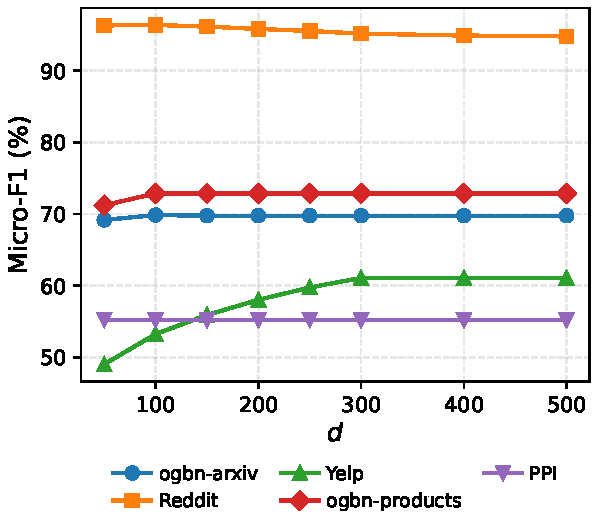
\includegraphics[width=\linewidth]{figures/sens_dim_croped.pdf}
    \caption{$d$}\label{fig_2_a}
  \end{subfigure}\hfill
  \begin{subfigure}[b]{0.3\linewidth}
    \centering
    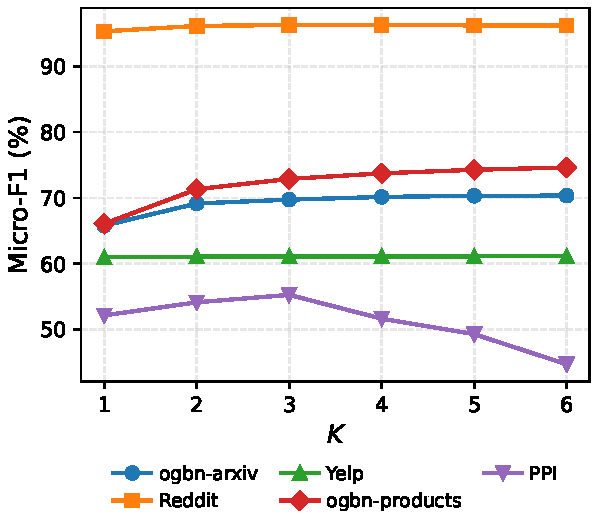
\includegraphics[width=\linewidth]{figures/sens_K_croped.pdf}
    \caption{$K$}\label{fig_2_b}
  \end{subfigure}\hfill
  \begin{subfigure}[b]{0.3\linewidth}
    \centering
    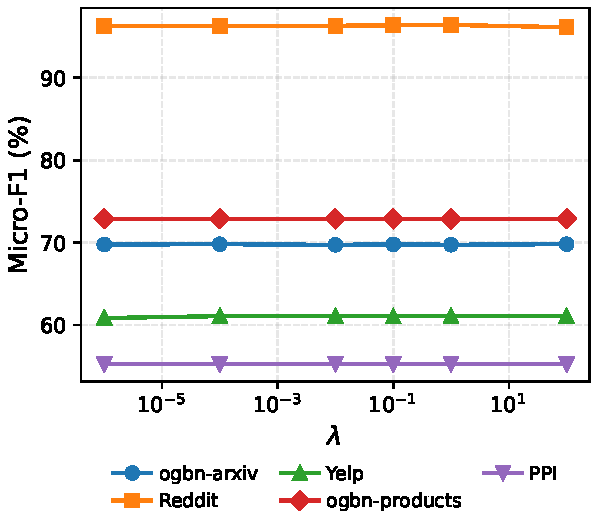
\includegraphics[width=\linewidth]{figures/sens_lamb_croped.pdf}
    \caption{$\lambda$}\label{fig_2_c}
  \end{subfigure}
  \caption{Performance of GW-CCA versus $d$, $K$, $\lambda$ on node classification (Micro-F1, \%).}
  \label{fig_2}
\end{figure}

\end{document}
